\begin{frame}
  \frametitle{\problemtitle}
  \begin{block}{Problem}
    Construct a valid \emph{Pentominous} grid of a given size:
    \begin{itemize}
      \item Divide an $h\times w$ grid into regions of size $5$ (pentominoes)\dots
      \item \dots such that no two adjacent regions have the same shape.
    \end{itemize} 
  \end{block}
  \vspace{5mm}
  \centering
  
\includegraphics[width=0.45\textwidth]{03}
\end{frame}
\begin{frame}
  \frametitle{\problemtitle}
  \begin{block}{Insights and corner cases}
    \begin{itemize}
      \item<+-> One of $h$ or $w$ must be a multiple of $5$; by symmetry, assume it's $w$.
      \item<+-> $1 \times w$ is only solvable for $w = 5$:
        \begin{center}
          
\includegraphics[height=5mm]{1_5}
          \hspace{10mm}
          
\includegraphics[height=5mm]{1_10}
        \end{center}
      \item<+-> $2 \times 5$ is not solvable:
        \begin{center}
          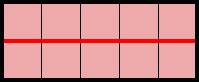
\includegraphics[height=10mm]{2_5a}
          \hspace{10mm}
          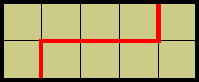
\includegraphics[height=10mm]{2_5b}
          \hspace{10mm}
          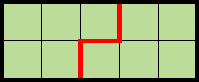
\includegraphics[height=10mm]{2_5c}
        \end{center}
      \item<+-> $2 \times w$ is solvable in all other cases:
        \begin{center}
          \includegraphics<4>[height=10mm]{2_10}
          \includegraphics<5>[height=10mm]{2_15}
          \includegraphics<6->[height=10mm]{2_20}
        \end{center}
    \end{itemize}
  \end{block}
\end{frame}
\begin{frame}
  \frametitle{\problemtitle}
  \begin{block}{Solution}
    \begin{itemize}
      \item<+-> For $3\times 5$ we can come up with a solution that can be repeated to achieve any width:
        \begin{center}
          \includegraphics<1>[height=15mm]{3_5}
          \includegraphics<2>[height=15mm]{3_10}
          \includegraphics<3->[height=15mm]{3_15}
        \end{center}
        \pause\pause
      \item<+-> Similar repeatable patterns exist for heights $4$, $5$, $6$ and $7$:
        \begin{center}
          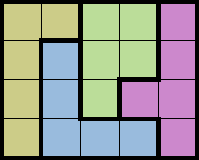
\includegraphics[height=16mm]{4_5}
          \hspace{8mm}
          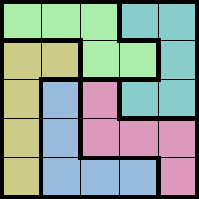
\includegraphics[height=20mm]{5_5}
          \hspace{8mm}
          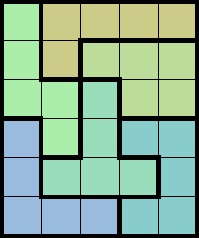
\includegraphics[height=24mm]{6_5}
          \hspace{8mm}
          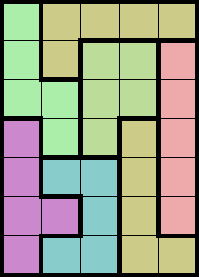
\includegraphics[height=28mm]{7_5}
        \end{center}
    \end{itemize}
  \end{block}
\end{frame}
\begin{frame}
  \frametitle{\problemtitle}
  \begin{block}{Solution (continued)}
    \begin{itemize}
      \item<+-> With some care, these patterns can be chosen so that they tile along both directions:
        \begin{center}
          \includegraphics<1>[height=12mm]{3_5}
          \includegraphics<2>[height=12mm]{3_10}
          \includegraphics<3>[height=12mm]{3_15}
          \includegraphics<4>[height=32mm]{8_15}
          \includegraphics<5->[height=52mm]{13_15}
        \end{center}
        \pause\pause\pause\pause
      \item<+-> This way, we can reduce any height $h$ to one of the base cases $3$, $4$, $5$, $6$ or $7$.
    \end{itemize}
  \end{block}
\end{frame}
